\chapter{Background}
\label{ch:background}
This chapter presents basic theory and techniques behind search engines. First
the software used in the implementation are explained, and then followed by a
detailed description on how the documents are scored inside the search engine from a
query. Finally, relevance feedback is described as well as how it may be used with query
expansion.

\section{Open Source Search Engine Solutions}
Making large amounts of data available for users to search requires speialized search engines.

At the time of writing there exists open source alternatives like Elasticsearch\footnote{\url{https://www.elastic.co/products/elasticsearch}},
Solr\footnote{\url{http://lucene.apache.org/solr/}} and Xapian\footnote{\url{https://xapian.org/}}.

Some of the search engines contains query expansion implementations,
but they are limited to synonyms expansion.
% None of the open source databases deliver personalized search capabilities.

\section{Software}
This section describs the software used in this master thesis.
Lucene were used in the initial implementation of query expansion.
The last experiment utilized Node.JS as the webserver and Elasticsearch as the search engine.

\subsection{Node.js}
Node.js\footnote{\url{https://nodejs.org}} version 7 was chosen as the webserver.
Node.js was chosen because the author has knowledge of the technology,
and it contains a rich package manager called NPM.
By utilizing open source libraries through NPM, more time could be spent implementing the algoritms for query expansion.
Inside NodeJS lies the V8\footnote{\url{https://developers.google.com/v8/}} JavaScript engine.

\subsection{Lucene}
Lucene\footnote{\url{https://lucene.apache.org/}} is an open-source full-text search engine library written in Java.
According to Lucene\footnote{\url{http://lucene.apache.org/core/}} the index size is only about 20-30\% of the original text.
Lucene's search features features such as ranked search, field search and faceting, to mention a few.

Lucene exposes the low level API's which gives very much control over the inner workings of Lucene.
Table \ref{tbl:inverted-index} shows a low level data structure inside Lucene called an inverted index.
The table contains a list of all the possible terms inside a text.
The second column is the frequency each term has.
Lastly, the documents column list all the documents where the given term occurs.
An inverted index requires more resources when indexing,
but the data structure are effective when searching.
The query expansion which is used in this master thesis requires information stored in the inverted index.

To illustrate how the inverted index works, Lucene recieves a query for the terms \texttt{blue}.
Using table \ref{tbl:inverted-index} the inverted index shows that the term has a frequency of three,
and that the term occurs in document 1, 2 and 3.
A search result would then return document 1, 2 and 3.

One important drawback with Lucene is that it is not scalable across multiple machines.
However, scalable across multiple machines are on of the advantages of using Elasticsearch.

\begin{table}[h]
    \centering
    \begin{tabular}{l|l|l}
    Term   & Frequency & Documents                                                 \\ \hline
    blue   & 3         & Document 1, document 2, document 3                        \\
    sky    & 1         & Document 2                                                \\
    clouds & 4         & Document 2, document 3, document 4, document 5            \\
    rain   & 2         & Document 2, document 5                                    \\
    plane  & 2         & Document 1, document 4                                    \\
    sunset & 5         & Document 1, document 2, document 3, document 4 document 5 \\
    \end{tabular}
    \caption{Example of an inverted index inside Lucene}
    \label{tbl:inverted-index}
\end{table}


\subsection{Elasticsearch}
Elasticsearch\footnote{\url{https://www.elastic.co/products/elasticsearch}} v5 were used as the search engine in the implementation described in this master thesis.
Elasticsearch has proven the ability to scale up to petabytes of data \cite{elasticsearch-scale}.
Elasticsearch is open source and built on top of Lucene.
Lucene is the search engine itself,
and Elasticsearch provides functionality for distribution and a REST API interface.

The following topics describes basic termonology used in Elasticsearch.
This information is needed to understand some of the results and observations,
and the implementation described in chapter \ref{ch:approach} and chapter \ref{ch:evaluation}.

\subsubsection{Cluster}
One or more servers connected together is called a cluster.
Elasticsearch indices are divided into shards which are distributed across the servers in the cluster.
Queries is also distributed to all the servers in the cluster, which again increases the performance.
Elasticsearch is responsible for distributing the shards across the physical servers,
and makes sure that replica shards are not on the same physical server.
The cluster used in this master thesis consisted of one server.

\subsubsection{Node Types}
Elasticsearch have four different node types: master node, data node, ingest node and tribe node.
The master node is responsible of handling administrative cluster tasks such as:
creating or deleting an index, tracking online and offline nodes and deciding how the shards should be distributed.
Data nodes is responsible for holding the shards and executing queries.
Ingest nodes is used as pre-processing nodes.
A tribe node is handling the coordination of querying and indexing.
Tribe nodes i also known as coordination nodes.
All nodes in a cluster is also an coordination node.


\subsubsection{Sharding}
The stored data in Elasticsearch may grow to become larger than the hardware on a single machine can handle,
both in size and in number of requests.
To mitigate the problem elasticsearch splits each index into multiple segments called shards.
Each of this shards may be distributed across multiple nodes.
This leads to higher performance when indexing new documents and when searching the documents.
The shards may also be duplicated to support higher query volumes and availability.

There is important distinction between an Elasticsearch index and a Lucene index.
A Lucene index, is the index which contains the inverted indices and holds all the data.
An Elasticsearch index on the other hand consists of on or more shards.
One Elasticsearch shard is the same as a Lucene index.

However, when the cluster consists of multiple nodes a query strategy is required.
Figure \ref{fig:elasticsearch-sharding} illustrates how an index may be distributed across three nodes.
The figure shows a simplified view on how a query are distributed across three nodes.
First the query arrives a coordination node.
The coordination node parses the query and determines which nodes holds shards for the given index.
Each shard determines locally which documents are most relevant from the query.
Metada from all the shards are then sent back to the coordination node.
On the coordination node alle the retrieved metadata are used to calculate the global result.
After the global result have been calculated,
all the shards are then queried for the documents from the global result.
After the documents are retrieved the result are returned back to the client.

\begin{figure}[h]
  \centering
  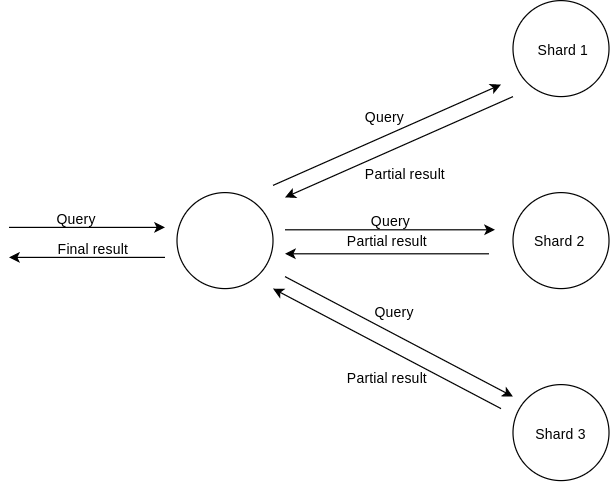
\includegraphics[width=0.9\linewidth]{img/elasticsearch-sharding.png}
  \caption{Elasticsearch distributing query agains all the shards}
  \label{fig:elasticsearch-sharding}
\end{figure}

\subsubsection{Aproximate Values}
As a result of Elasticsearch's distributed nature some queries will return estimated values.
Aggregations in Elasticsearch is an example which may return estimated values.

Table \ref{tbl:shard-term-counts} has a list of words across three different shards.
The term frequencies are listed inside the parenthesis.
When a client queries for the top three terms, the query is distributed to the shards.
Each shard then returns their local top three terms.
Given Table \ref{tbl:shard-term-counts},
the shards will return the terms listed in table \ref{tbl:shard-top}.
On the coordination node the global top three terms are calculated.
The top three terms is listed in table \ref{tbl:final-result}, which are \texttt{blue}, \texttt{sky} and \texttt{clouds}.
However, \texttt{blue}, \texttt{sky} and \texttt{clouds} are not the actual top three terms.
If the coordination node had all the knowledge in table \ref{tbl:shard-term-counts},
the top three terms would be \texttt{blue}, \texttt{sky} and \texttt{insta},
with the term frequencies 60, 32 and 22 respectively.
With global knowledge both the frequencies and one of the top 3 terms have changed.

The example explained above is exaggerated to illustrate what might happen in Elasticsearch's distributed architechture.
Even though the result is not exact, it is good enough for most use cases.
Elasticsearch can be configured to return more exact results,
at the cost of longer response times.

\begin{table}[h!]
    \centering
    \begin{tabular}{|l|c|c|c|}
    \hline
    ~ & \textbf{Shard 1}    & \textbf{Shard 2}     & \textbf{Shard 3}    \\ \hline
    1 & blue (10)  & blue (20)   & blue (30)  \\ \hline
    2 & clouds (9) & clouds (12) & sky (25)   \\ \hline
    3 & sky (5)    & insta (5)   & insta (15) \\ \hline
    4 & plane (4)  & plane (3)   & plane (10) \\ \hline
    5 & insta (2)  & sky (2)     & rain (3)   \\ \hline
    \end{tabular}
    \caption{Term list with the corresponding term count.}
    \label{tbl:shard-term-counts}
\end{table}

\begin{table}[h!]
    \centering
    \begin{tabular}{|l|c|c|c|}
    \hline
    ~ & \textbf{Shard 1}    & \textbf{Shard 2}     & \textbf{Shard 3}    \\ \hline
    1 & blue (10)  & blue (20)   & blue (30)  \\ \hline
    2 & clouds (9) & clouds (12) & sky (25)   \\ \hline
    3 & sky (5)    & insta (5)   & insta (15) \\ \hline
    \end{tabular}
    \caption{Term list of the top three terms returned to the coordination node.}
    \label{tbl:shard-top}
\end{table}

\begin{table}[h!]
    \centering
    \begin{tabular}{|l|c|}
    \hline
    ~ & \textbf{Returned result} \\ \hline
    1 & blue (60)     \\ \hline
    2 & sky (30)    \\ \hline
    3 & clouds (21)       \\ \hline
    \end{tabular}
    \caption{Top three terms which are returned back to the client.}
    \label{tbl:final-result}
\end{table}

https://www.elastic.co/guide/en/elasticsearch/reference/current/search-aggregations-bucket-terms-aggregation.html

\section{Basic Search Engine Concepts}
A common approach for search engines is to use \textit{term frequency} (TF) and \textit{inverse document frequency} (IDF) to calculate a document\'s relevance based on a query.
Documents with the highest TF from a query, are believed to be the most relevant.
On the other hand, the most common words are removed as they do not contain information about the topic.
TF and IDF alone is a simple model, and Elasticsearch uses a more sophisticated model.
Elasticsearch's document scoring model is described in the following subsections.
This section describes how Elasticsearch scores its documents and is based on the documentation found on the website \cite{elasticsearch-scoring}.

\subsection{Term Frequency}
Term frequency is the number of times a term is mentioned in a document.
A document containing a term multiple times is probably more relevant than a document containing fewer occurences.
However, in this work a term is only present once in each document, and the reason is described in greater detail in Chapter \ref{ch:approach}.
Term frequency calculation is given by Equation \ref{eq:term-frequency}.

\begin{cequation}[H]
	\begin{equation}
		\mathbf{tf} = \sqrt{frequency}
	\end{equation}
	\caption{Term frequency calculation in Elasticsearch.}
  \label{eq:term-frequency}
\end{cequation}

\subsection{Inverse Document Frequency}
Inverse document frequency describes how many times a term is present in all the documents.
Terms with high frequencies are often less relevant.
E.g. the terms "a" and "an" often appear in a sentence, but should not be given a high score even though they appear numerous times.
\begin{cequation}[H]
	\begin{equation}
		\mathbf{idf} = 1 + \log{[\frac{numDocs}{docFrequency + 1}]}
	\end{equation}
	\caption{Inverse Document Frequency calculation in Elasticsearch.}
  \label{eq:idf}
\end{cequation}

\subsection{Document Normalization}
A title field is likely to be shorter compared to a description field.
As a result, the description field possibly contains more instances of a given term.
To account for longer fields, document normalization is used.
Elasticsearch's implementation is illustrated in equation \ref{eq:normalization}.

\begin{cequation}[H]
	\begin{equation}
		\mathbf{normalization} = \frac{1}{\sqrt{numTerms}}
	\end{equation}
	\caption{Normalization.}
  \label{eq:normalization}
\end{cequation}

\subsection{Document Score}
\label{sec:doc-score}
After calculating term frequency, inverse document frequency and document normalization, the factors are multiplied together.
A document's score in Elasticsearch is given by the Equation \ref{eq:document-score}.

\begin{cequation}[H]
	\begin{equation}
		\mathbf{documentScore} = tf \times idf \times normalization
	\end{equation}
	\caption{Final document score.}
  \label{eq:document-score}
\end{cequation}

\subsection{Vector Space Model}
The theory presented earlier only describes how to score a single term, but user queries may contain multiple terms.
Search engines often apply a technique called \textit{Vector Space Model} on queries with multiple terms.
The vector space model represent the query and the document as vectors.
The vector is a an array which holds term weights.
Vector similarity is calculated between the query and the documents.
The documents which are most similar is then returned from the search.
The most common technique to calculate similarity is called cosine similarity.

\subsection{Multiple Term Query}
Elasticsearch's underlying technology Lucene,
combines the boolean model, TF/IDF and vector space model to score queries with multiple terms against documents \footnote{\url{https://www.elastic.co/guide/en/elasticsearch/guide/current/practical-scoring-function.html}}.
Equation \ref{eq:scoring-function} shows how each document is scored against a multiterm query.
Table \ref{tbl:scoring-function} explains each variable in equation \ref{eq:scoring-function}.

The variables \textit{queryNorm}, \textit{coord} and \textit{getBoost} are described in greater details in the following paragraphs.
\textit{queryNorm} or \textit{query normalization factor} are used to make results from different queries comparable.
The factor is calculated using equation \ref{eq:query-normalization-factor}.
\textit{sumOfSquaredWeights} is determined by adding the idf value of all the terms in the query,
and squaring the result afterwards.
As a result, every document will have the same query normalization factors.

The \textit{coord} variable stands for \textit{coordination factor}.
With the factor, documents which contain most terms from the query will be ranked highest.
Without the factor documents with more matching terms would still be ranked higher.
However, the boost factor gives documents with more matching terms an even higher score compared to documents with less matching terms.
For instance, a query might contain two terms, with a term weight of 3.
If the score where calculated without the boost factor,
documents with one matching term would recieve a score of 3 and documents with two matching terms would recieve a score of 6.
Calculating the score with the boost factor, documents with one matching term recieves a score of $(3 \times 1)/ 2 = 1.5$,
and documents with two matching terms recieve a score of $(6 \times 2) / 2 = 6$.

Lastly, the variable named \textit{getBoost} is used to make some field impact more on the document score,
compared to other fields.
In Elasticsearch there are two different methods of boosting: query time boosting and index time boosting.
Index time boosting means that all terms in a specified field, will recieve the boost factor during indexing.
Query time boosting, on the other hand, calculates and adds the boost factor when the query is running on the Elasticsearch node.

\begin{cequation}
	\begin{equation}
		\begin{aligned}
			\mathbf{queryNorm} = \frac{1}{\sqrt{sumOfSquaredWeights}}
		\end{aligned}
	\end{equation}
	\caption{Equation for calculating the query normalization factor}
  \label{eq:query-normalization-factor}
\end{cequation}

\begin{cequation}
	\begin{equation}
		\begin{aligned}
			\mathbf{score(q,d)} = & coord(q,d) \times queryNorm(q) \\
														& \times \sum tf(t in d) \times idf(t)^2 \times t.getBoost() \times norm(t,d)
		\end{aligned}
	\end{equation}
	\caption{Equation for scoring documents when searching with multiple terms. Each variable is described in table \ref{tbl:scoring-function}.}
  \label{eq:scoring-function}
\end{cequation}

\begin{table}
		\centering
    \begin{tabular}{|l|l|}
    \hline
		\multicolumn{1}{|c|}{\bfseries Variable} & \multicolumn{1}{c|}{\bfseries Description} \\ \hline
    \textit{t}         & term                           		\\ \hline
    \textit{d}         & document                       		\\ \hline
    \textit{q}         & query                          		\\ \hline
		\textit{score}     & document score from a given query	\\ \hline
    \textit{coord}     & coordination factor            		\\ \hline
    \textit{queryNorm} & query normalization factor     		\\ \hline
    \textit{tf}        & term frequency                 		\\ \hline
    \textit{idf}       & inverse document frequency     		\\ \hline
    \textit{getBoost}  & boost factor used on the query 		\\ \hline
    \textit{norm}      & document normalization factor  		\\ \hline
    \end{tabular}
		\caption{Variable descriptions for equation \ref{eq:scoring-function}.}
		\label{tbl:scoring-function}
\end{table}

%\section{Relevance}
Should I have a separate section about relevance?

\section{Relevance Feedback}
The idea behind \textit{relevance feedback} is to use the result from the initial query to extract relevant information from the top-k documents.
Once the information is extracted, a new query is executed with extracted information.
Results from the second query are returned to the user.
The assumption is that the second query returns documents which are more relevant to the user.

In \cite{ir-book} the authors define \textit{relevance feedback} as: "when the user explicitly provides information on relevant documents to a query,"
and \textit{query expansion} as: "when information related to the query is used to expand it" \cite[p. 177]{ir-book}.
In other words to use \textit{relevance feedback}, input from the user is needed.
For example the user could be given the task to mark whether the documents are relevant or not.
In practice it is often difficult for a user to determine the result's relevance.
For \textit{query expansion} information like position and tags may be used to expand the query.
A more detailed explanation of query expansion is described in section \ref{sec:query-expansion}.

\textit{Relevance feedback} is divided into three main categories \textit{explicit feedback}, \textit{implicit feedback} and \textit{pseude-relevance feedback},
and is introduced in the next two subsections.

\subsection{Explicit vs Implicit Feedback}
\textit{Explicit feedback} data are retrieved directly from user interaction.
An example would be if the user selects the section "graphic cards" in an online store.
From the interaction the user explicitly states that the search should only contain graphic cards.
Another approach is to use data from a user search.
If a user clicks on a search result, the result may be regarded as relevant.
Even though the result may not be relevant, it is a good indication.
The problem with explicit feedback, is that it requires interaction from the user.

\textit{Implicit feedback} on the other hand, does not require any involvement from the user.
Examples of implicit user data are collecting the documents from a search result that  are opened by a user,
and measure time spent viewing a document.

\subsection{Pseudo-Relevance Feedback}
Retrieval of data to use relevance feedback requires either explicit or implicit user interaction.
Manually involving the user in the search is undesireable.
To avoid this, an approach called pseudo-relevance feedback can be used.
Using implicit feedback requires a system which does the data collection and post process the information.
Pseudo-relevance, on the other hand, uses information from the first search, and thus leads to a simpler implementation.

Often the top-k documents are used to find pseudo-relevance for query expansion.
However, the top-k documents are in many cases not relevant, and thus not suitable data for query expansion \cite{pseudo-relevance-invalid}.
Section \ref{sec:query-expansion} describes a method to extract information from the top-k documents which is regarded as relevant information.

\section{Query Expansion}
\label{sec:query-expansion}
When a user searches using the query "Super Bowl" the day after the sport event has taken place,
it is likely that the user wants information about the event from the previous day.
The query "Super Bowl" is likely to also return documents from previous years.
If the search engine could be able to notice that recent documents also contains the term "2016,"
the extra term could be added to the query.
The new query "Super Bowl 2016" is likely to rank documents from this year's Super Bowl higher, as a result of the extra term.
This technique is called query expansion.

The idea behind query expansion is to add more terms to the user's query, and then use the extended query on the search engine.
According to literature, a query expanded search does improve the results \cite[ch. 5]{ir-book}.
Even though research shows promising results, query expansions require explicit information which in practice often is difficult to acquire.
In a free text search users expect to automatically recieve search results without having to answer questions or to filter the result to provide query expansion data.
On the other hand, according to Efron \cite{ir-hashtag}, hashtags provide an excellent way to acquire the explicit information needed for query expansion.

There are different methods of query expansion, and this report describes one technique called Kullback-Leibler divergence.
The implementation is described in chapter \ref{ch:approach}.

\subsection{Kullback-Leibler Divergence}
\textit{Kullback-Leibler divergence} (KL) measures how well distribution P(t) represents the distribution Q(t).
The variables in distribution P(t) and Q(t) are explained in the bullet points bellow.

\begin{itemize}
	\item \textit{numberOfTimesInTopKDocuments} is the number of times a term is present in the top-k documents
	\item \textit{numberOfTermsInTopKDocuments} is the number of terms in total in the top-k documents
	\item \textit{totalNumberOfTimesInCollection} is the total number of times a term is present in the data collection
	\item \textit{totalNumberOfTermsInCollection} is the total number of terms in the data collection
\end{itemize}

Equation \ref{eq:kl-distribution-p} explains how to calculate the distribution P(t),
and equation \ref{eq:kl-distribution-q} explains how to calculate distribution Q(t).

% Kullback-Leibler P distribution
\begin{cequation}[H]
	\begin{equation}
		\mathbf{P} = \frac{numberOfTimesInTopKDocuments}{numberOfTermsInTopKDocuments}
	\end{equation}
	\caption{}
  \label{eq:kl-distribution-p}
\end{cequation}

% Kullback-Leibler Q distribution
\begin{cequation}[H]
	\begin{equation}
		\mathbf{Q} = \frac{totalNumberOfTimesInCollection}{totalNumberOfTermsInCollection}
	\end{equation}
	\caption{}
  \label{eq:kl-distribution-q}
\end{cequation}

Computing the Kullback-Leibler divergence for a term is given by equation \ref{eq:kl-divergence}.

% Kullback-Leibler Distance Equation
\begin{cequation}[H]
	\begin{equation}
		\mathbf{KL}_D[P(t), Q(t)] = P(t)*\log{[\frac{P(t)}{Q(t)}]}
	\end{equation}
	\caption{Kullback-Leibler Divergence.}
  \label{eq:kl-divergence}
\end{cequation}

\subsubsection{Kullback-Leibler Divergence Example}
To illustrate how KL score is calculated, an example for the search term "sky" is displayed.
The expanded query may consist of up to 5 terms.
To keep this example short, only the top 5 terms are calculated and the term "sky" is excluded from the calculations.

Table \ref{tbl:kl-counts} contains information extracted using the data set described in section \ref{sec:dataset}.
Using equation \ref{eq:kl-divergence} and the information in table \ref{tbl:kl-counts}, the KL score for each term is calculated and is shown in table \ref{tbl:kl-score}.
The table \ref{tbl:kl-score} lists the terms descending according to their score.
From the original query we have the term "sky" and we may use 4 additional terms to complete the expansion.
The top 4 terms are "clouds", "2016", "blue" and "water",
which results in an expanded query containg the terms: "sky", "clouds", "2016", "blue" and "water".


\begin{table}
	\centering
    \begin{tabular}{|l|p{22mm}|p{22mm}|p{25mm}|p{25mm}|}
		\hline
    \textbf{Term}   & \textbf{numberOf- \newline TimesIn- \newline TopK- \newline Documents} &
		\textbf{numberOf- \newline TermsIn- \newline TopK- \newline Documents} &
		\textbf{totalNumber- \newline OfTimesIn- \newline Collection} &
		\textbf{totalNumber- \newline OfTermsIn- \newline Collection} \\ \hline
    blue   & 1                            & 42                           & 14                             & 298,962                         \\ \hline
    2016   & 2                            & 42                           & 143                            & 298,962                         \\ \hline
    clouds & 3                            & 42                           & 31                             & 298,962                         \\ \hline
    sea    & 1                            & 42                           & 34                             & 298,962                         \\ \hline
    water  & 1                            & 42                           & 24                             & 298,962                         \\ \hline
\end{tabular}
	\caption{The returned numbers for each of the top 5 terms excluding the term "sky".}
	\label{tbl:kl-counts}
\end{table}

\begin{table}
	\centering
    \begin{tabular}{|l|l|}
		\hline
    \textbf{Term}   & \textbf{Score}   \\ \hline
    clouds & 0.46678 \\ \hline
    2016   & 0.21908 \\ \hline
    blue   & 0.14836 \\ \hline
    water  & 0.13553 \\ \hline
    sea    & 0.12723 \\ \hline
    \end{tabular}
	\caption{KL divergence score of each term.}
	\label{tbl:kl-score}
\end{table}


\section{Notes}
- Personalized search Google https://googleblog.blogspot.no/2009/12/personalized-search-for-everyone.html
- Some of the queries from Elasticsearch returns estimated values (aggregations). Important because of performance. Queries is distributed across multiple nodes.
- Larger dataset equal incorrectness https://www.elastic.co/guide/en/elasticsearch/guide/current/relevance-is-broken.html
